\chapter{Evaluation}%
\label{cha:evaluation}

%As a rough outline, this chapter should address the following questions:
%\begin{itemize}
%   \item Which questions did you want to answer or which hypothesises did you want to test with the experiments?
%   \item Which metrics did you measure and how does their value relate to the questions you want to answer?
%   \item Which system parameters exist that may have an influence on the value on the metric? Which ones did you vary in your experiments? Intuitively, what are your expectations with regards to the relationship between the system parameters and the metrics?
%   \item How did the experiments that you did actually looked like, or how did you actually measure the chosen metrics?
%   \item What are the actual values that you measured in your experiments? Do they match your intuition about the relationship between the system parameters and the metrics?
%\end{itemize}

%\section{Auswertung der Testergebnisse}

%   \item Which questions did you want to answer or which hypothesises did you want to test with the experiments?
Zuerst einmal sollte im Rahmen dieser Arbeit geklärt werden, ob und wie Kontext kategorisiert werden kann. Untersucht wurde ebenfalls welche Kontextinformationen, zur Anpassung der Arbeitsabläufe eines IDS, verwendet werden können.  
%Ziele der Arbeit ist es zu evaluieren, ob sich die Leistung eines IDS verbessern lässt, wenn in Zugriffsentscheidungen Kontextinformationen miteinbezogen werden. Das Hauptaugenmerk liegt dabei darauf falsch-positive Meldungen zu verringern, und die Interpretierbarkeit der IDS-Logs zu erhöhen. Auch sollte untersucht wie gut sich die zur Verfügung stehenden Informationen in der gewählten Implementierung einbinden lassen. 
%   \item Which metrics did you measure and how does their value relate to the questions you want to answer? 
 Dabei wird zusätzlich beurteilt
%   \item Which system parameters exist that may have an influence on the value on the metric? Which ones did you vary in your experiments? Intuitively, what are your expectations with regards to the relationship between the system parameters and the metrics?

%   \item How did the experiments that you did actually looked like, or how did you actually measure the chosen metrics?

Die erhöhte Interpretierbarkeit wird durch die Kombina

%   \item What are the actual values that you measured in your experiments? Do they match your intuition about the relationship between the system parameters and the metrics?


%Zeek offers the best software/environment for the development of novel detection or processing techniques. It can be used for continuous monitoring of high-throughput networks. The scripting environment is extensible in a memory-safe language specialized in network data processing. It is not constrained by belonging to a single paradigm for network monitoring like the other tools.
Zeek bietet die beste Software/Umgebung für die Entwicklung neuer Erkennungs- oder Verarbeitungstechniken. Es kann für die kontinuierliche Überwachung von Netzwerken mit hohem Durchsatz verwendet werden. Die Skripting-Umgebung ist in einer speichersicheren Sprache erweiterbar, die auf die Verarbeitung von Netzwerkdaten spezialisiert ist. Im Gegensatz zu anderen Tools, ist es nicht auf ein einziges Paradigma für die Netzüberwachung limitiert.
\section{Mächtigkeit eines kontextsensitiven IDS}  
\section{Vergleich der Kontextkategorien} 
%\subsection{Theoretische Mächtigkeit einzelner Kategorien} 
\subsection{Verfügbarkeit der Informationen}
Die Informationen die ich in den definierten Kategorien als gegeben vorausgesetzt habe sind in der Praxis unterschiedlich schwer zu akquirieren. Offensichtlich ist es um ein Vielfaches einfacher korrekt die aktuelle Uhrzeit zu ermitteln als den Grund dafür das ein Nutzer eine Aktion ausführt zu bestimmen. Die nachfolgende Grafik dient dazu den meiner Einschätzung nach benötigten Aufwand zur Beschaffung einer Information zu veranschaulichen.
%TODO Grafik
\begin{figure}[H]
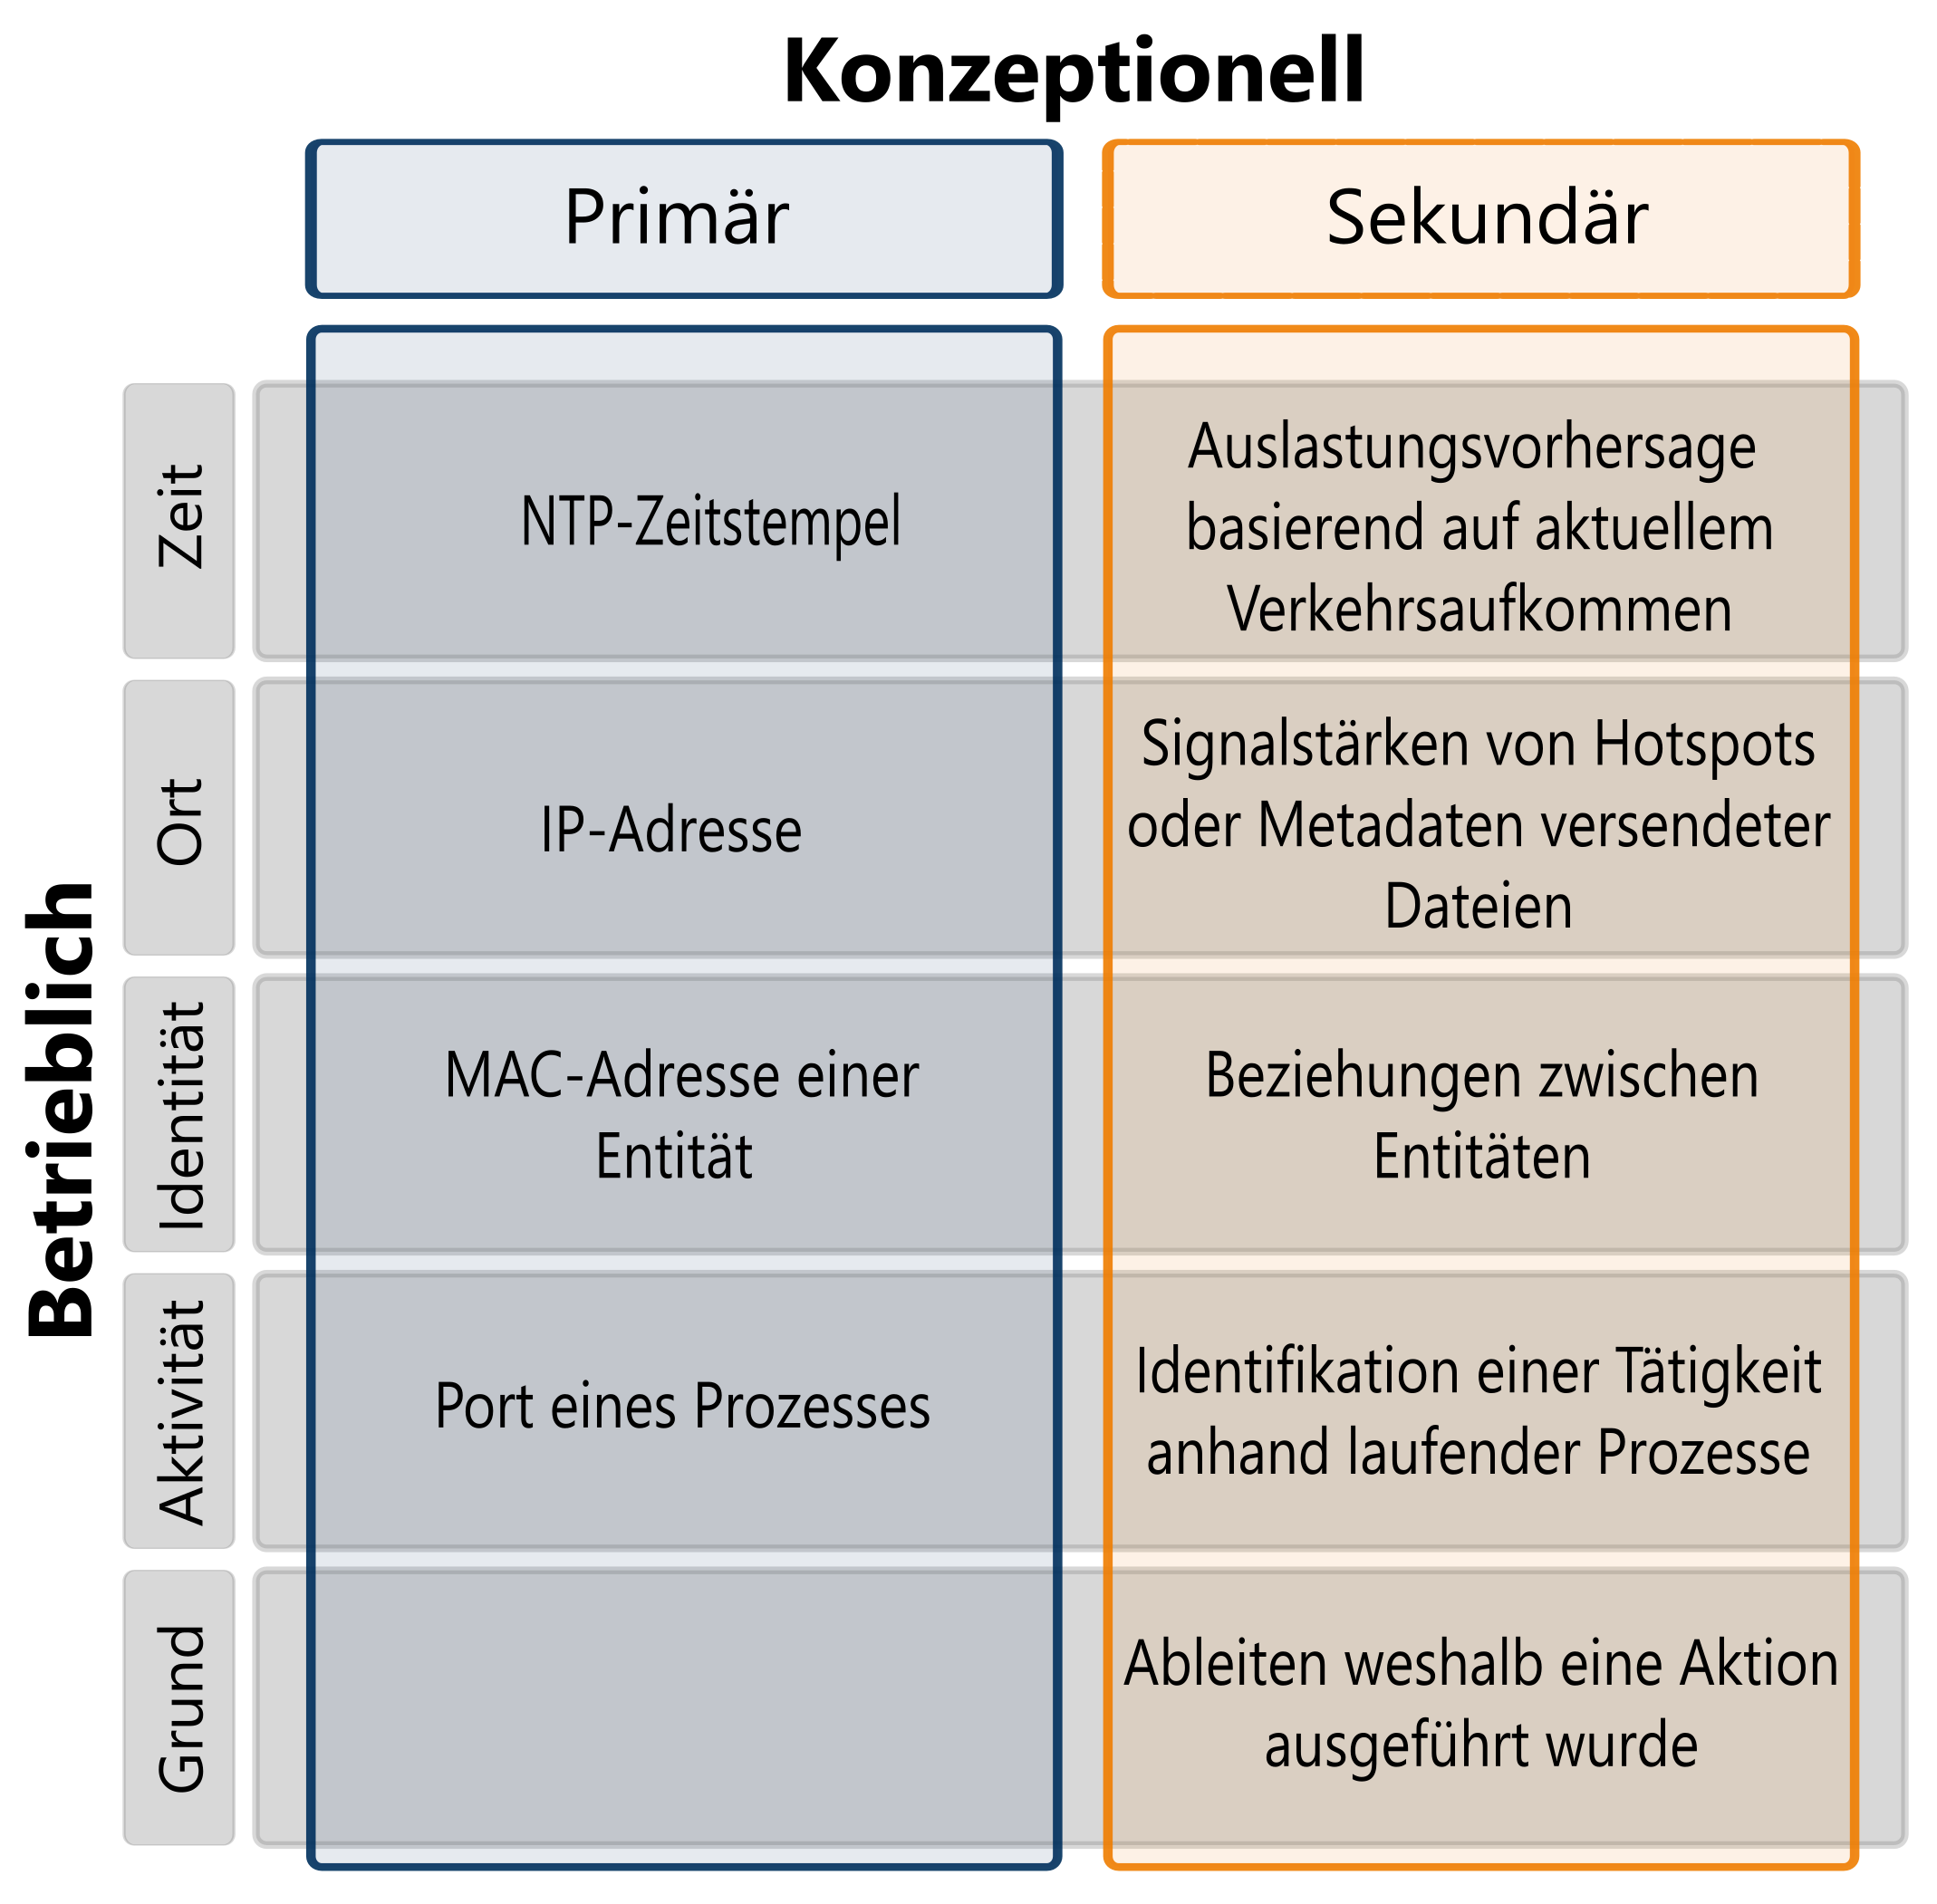
\includegraphics[width=15cm,height=15.2596cm]{graphic_1}
\caption{Placeholder}
\label{Placeholder}
\end{figure}
\begin{figure}[H]
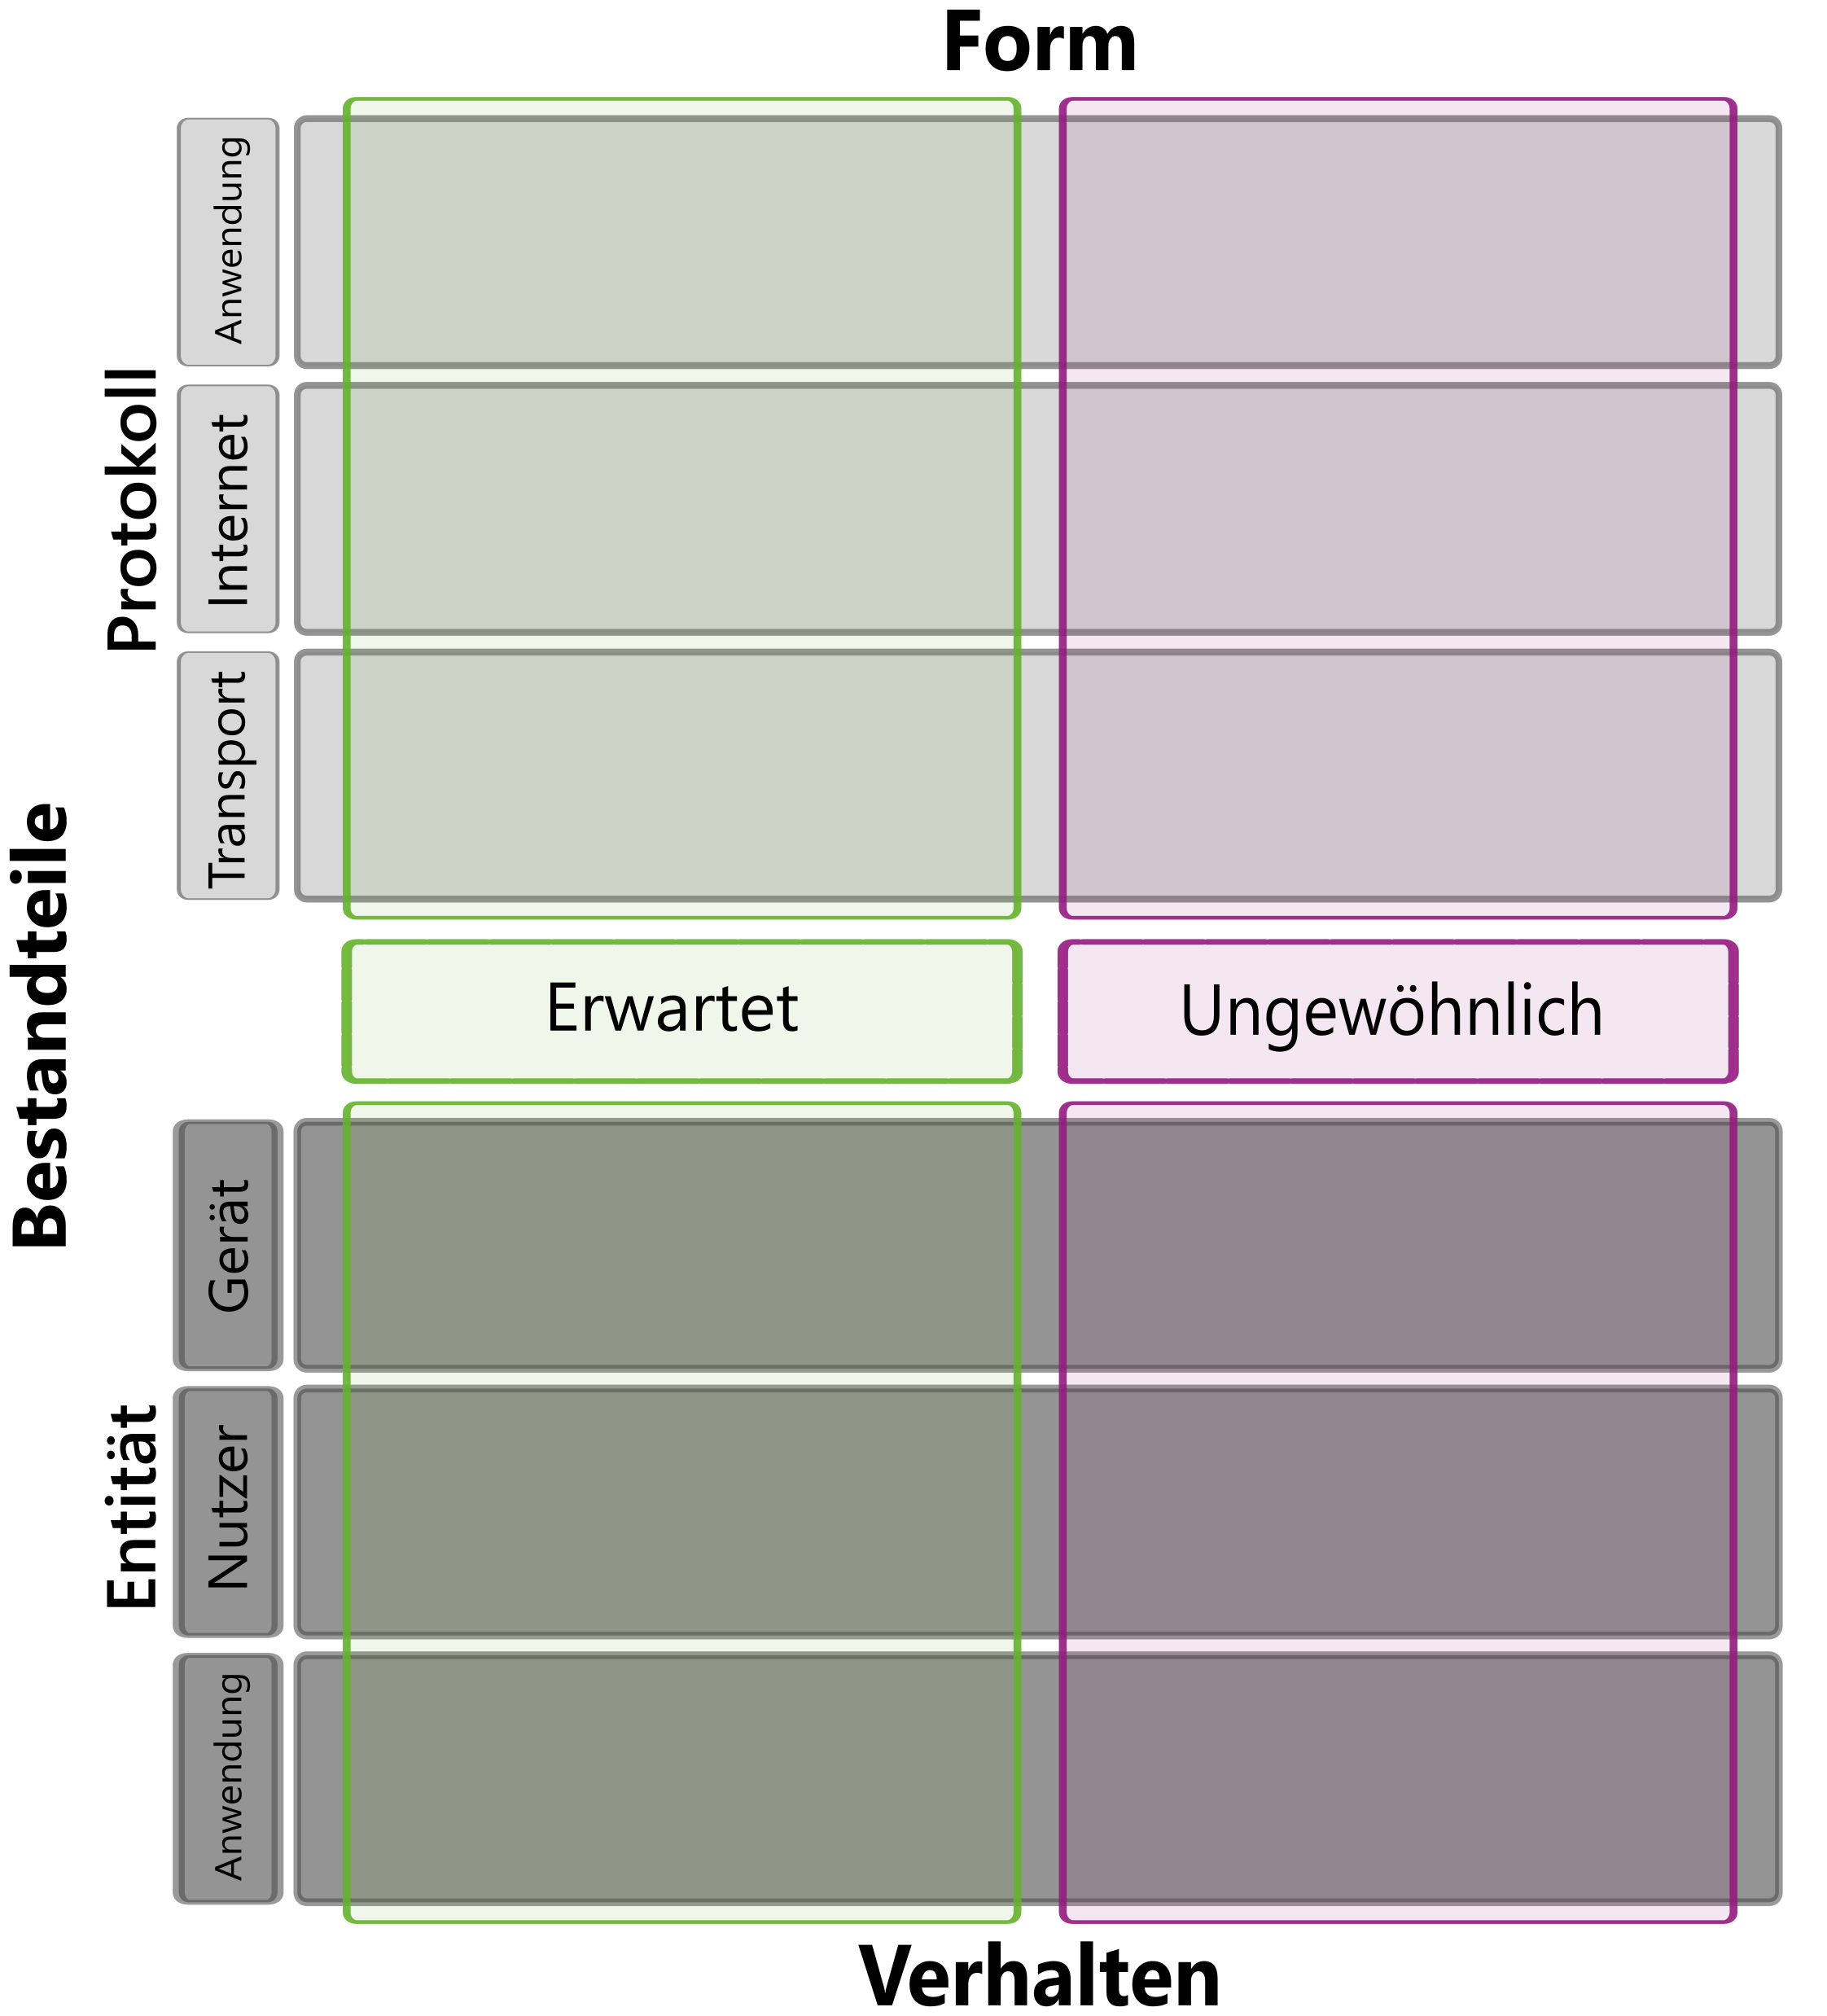
\includegraphics[width=15cm,height=16.97cm]{graphic_2}
\caption{Placeholder}
\label{Placeholder}
\end{figure}

\subsection{Qualität der Informationen}
Auch die Qualität der Informationen schwankt in der Praxis. Genauigkeit und Korrektheit der Informationen sind teils unterschiedlich. Auch die Vertrauenswürdigkeit und Aktualität der Akquirierungspunkte ist verschieden.
 

\begin{figure}[H]
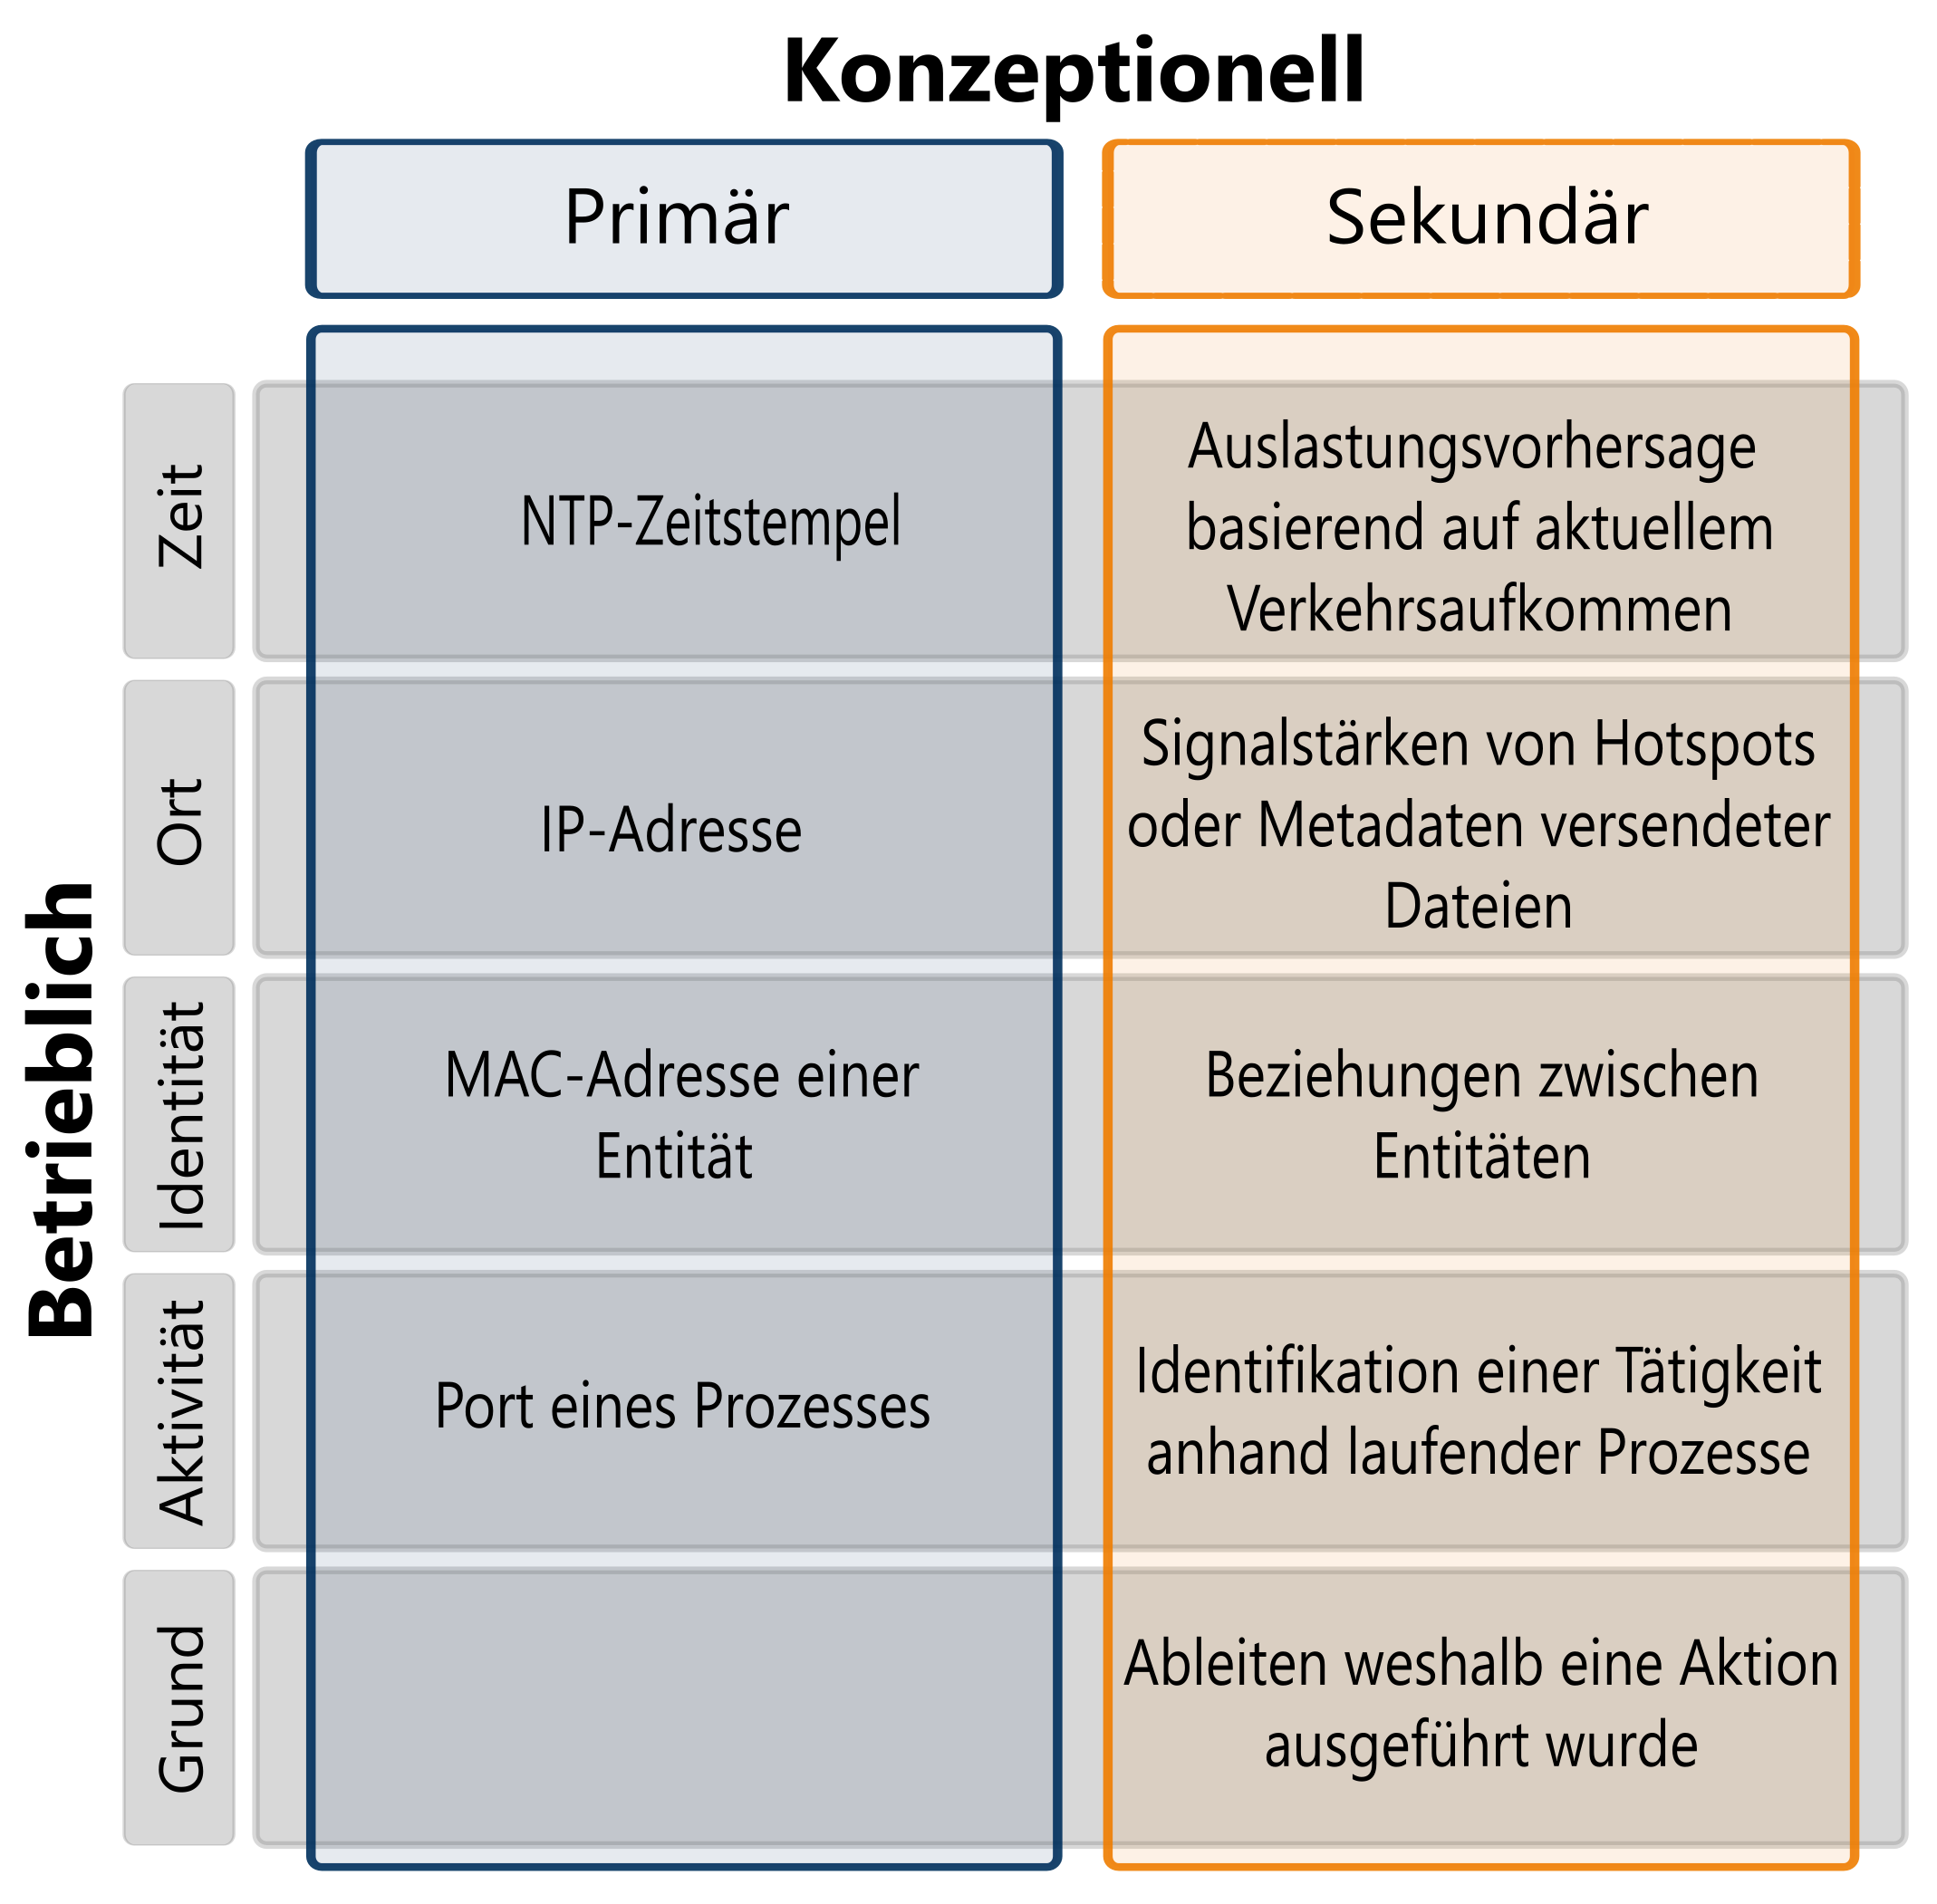
\includegraphics[width=15cm,height=15.2596cm]{graphic_1}
\caption{Placeholder}
\label{Placeholder}
\end{figure}
\begin{figure}[H]
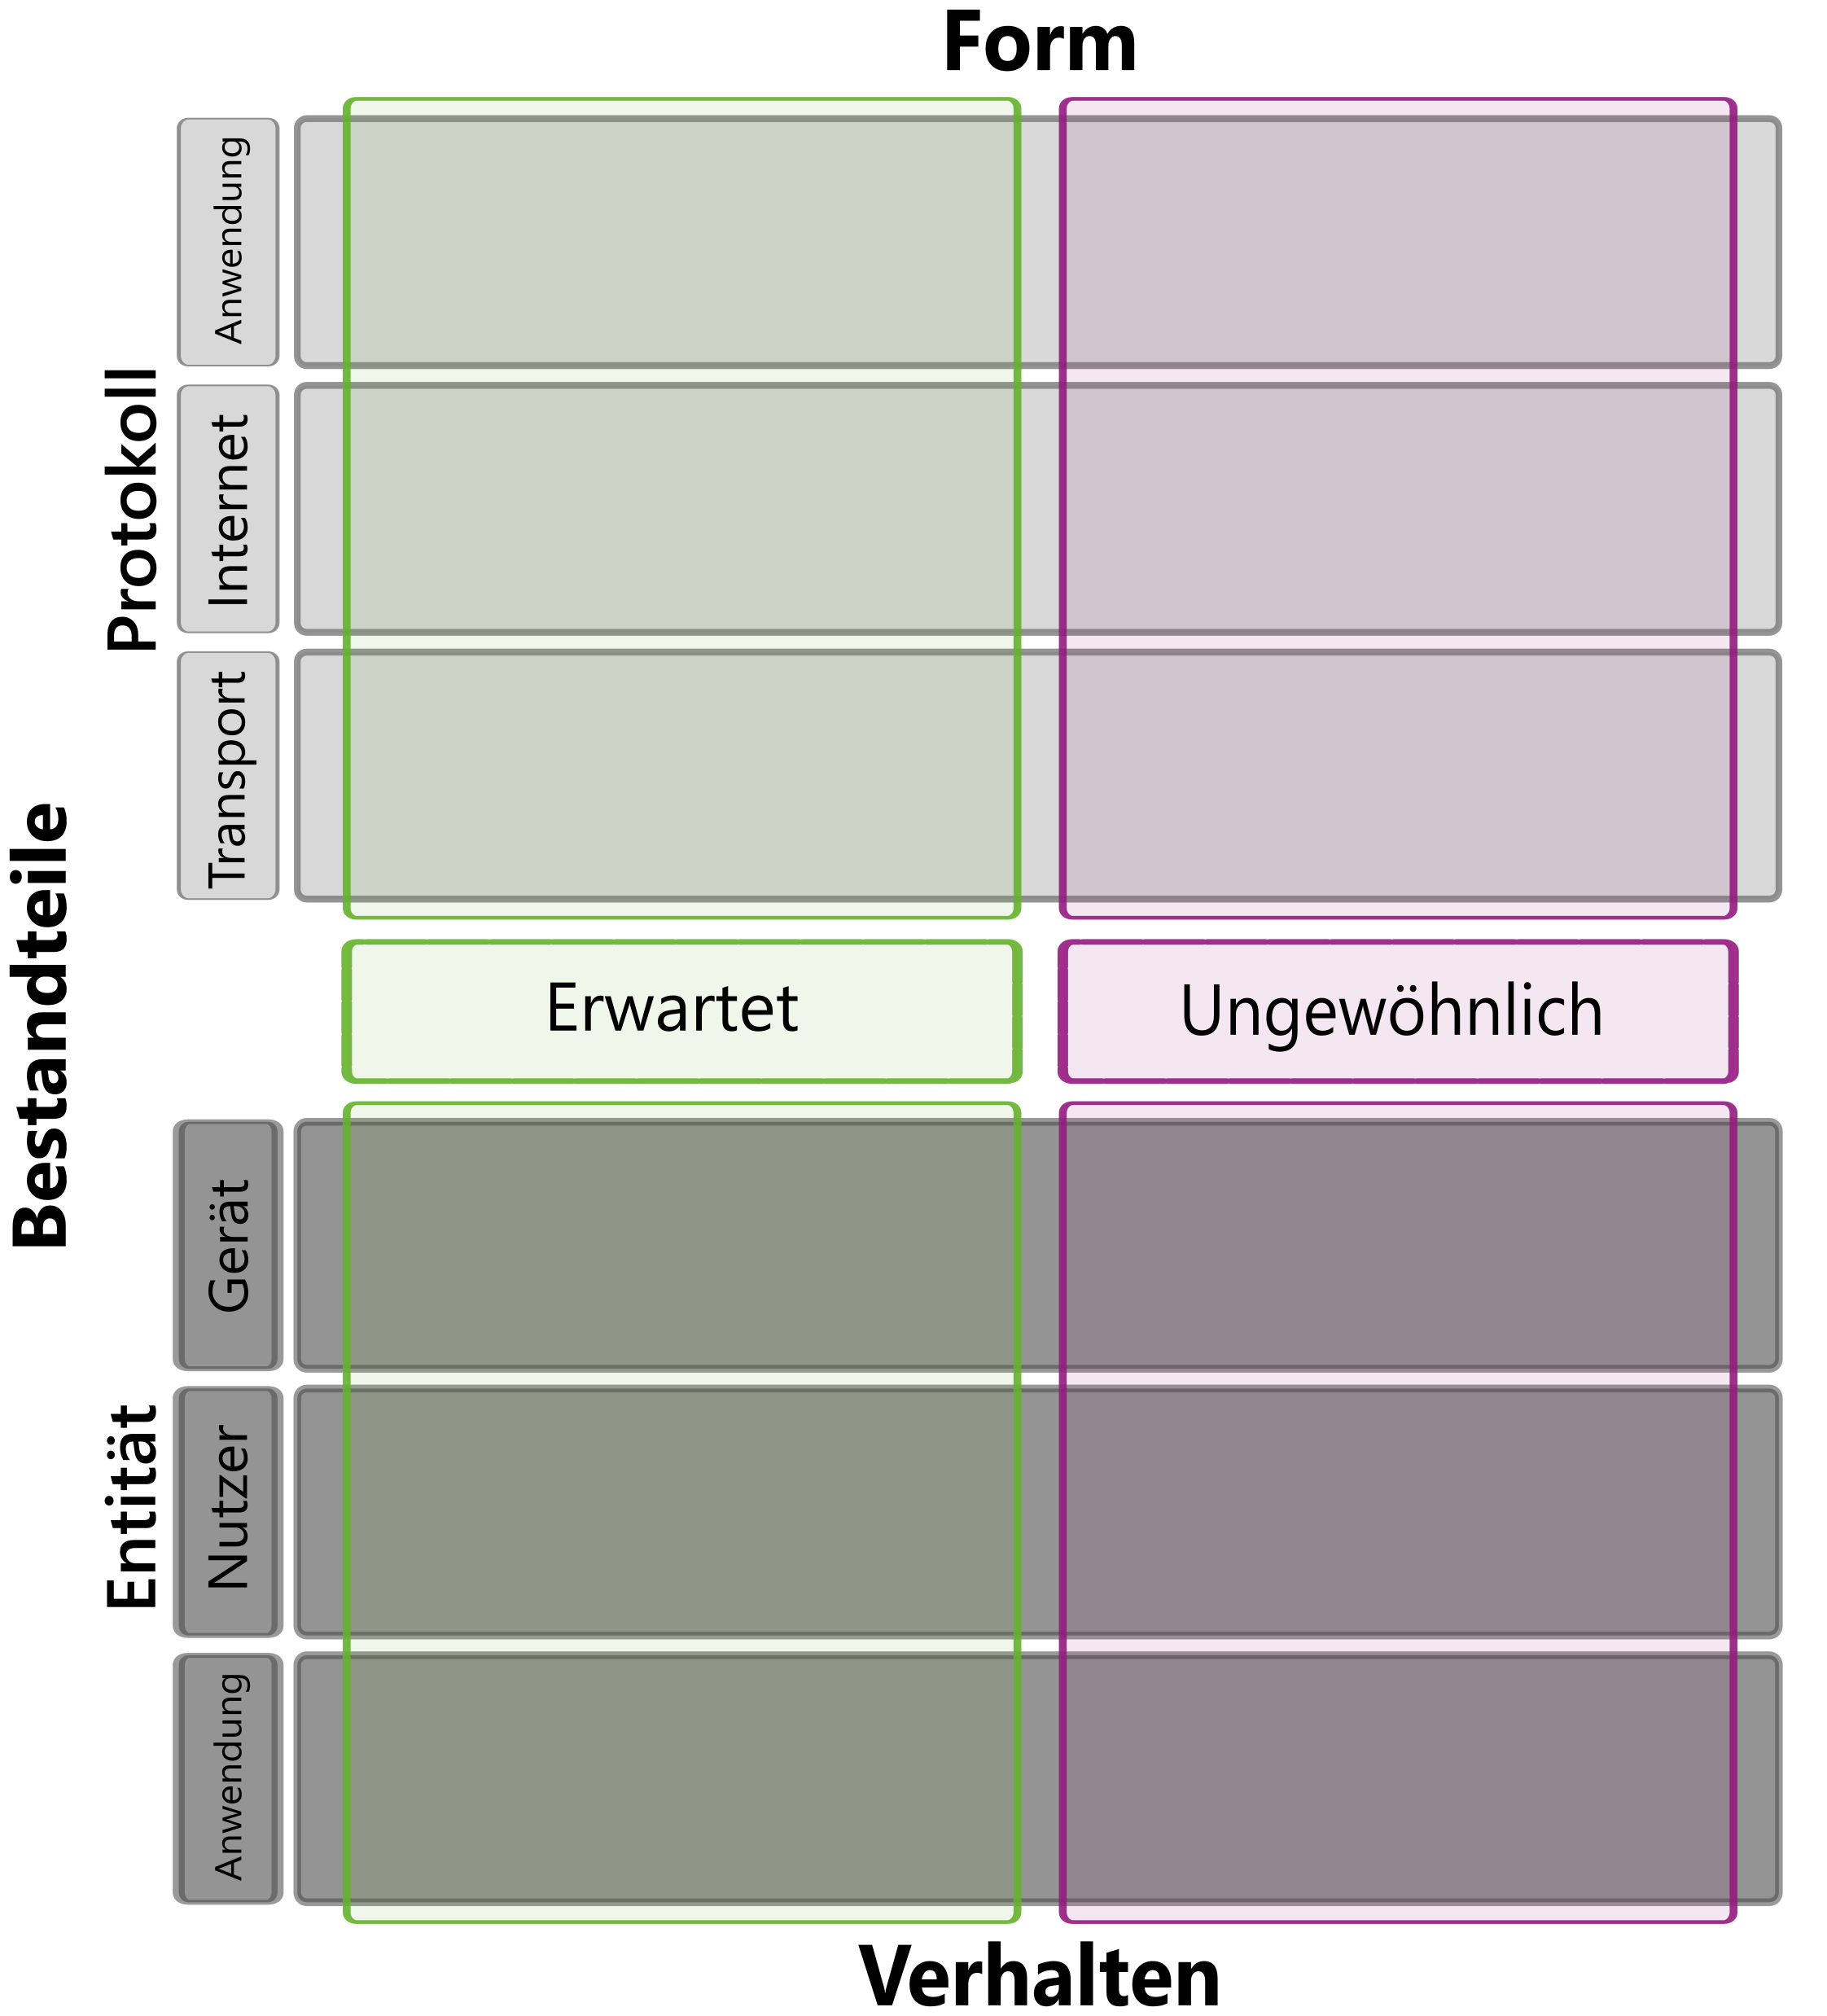
\includegraphics[width=15cm,height=16.97cm]{graphic_2}
\caption{Placeholder}
\label{Placeholder}
\end{figure}

\section{Leistungsverbesserung}
